
%(BEGIN_QUESTION)
% Copyright 2007, Tony R. Kuphaldt, released under the Creative Commons Attribution License (v 1.0)
% This means you may do almost anything with this work of mine, so long as you give me proper credit

Determine the directions of electric current where you see question marks in the following schematic diagram for a variable-speed AC motor drive, at the moment in time ($t_1$) specific on the oscillograph:

$$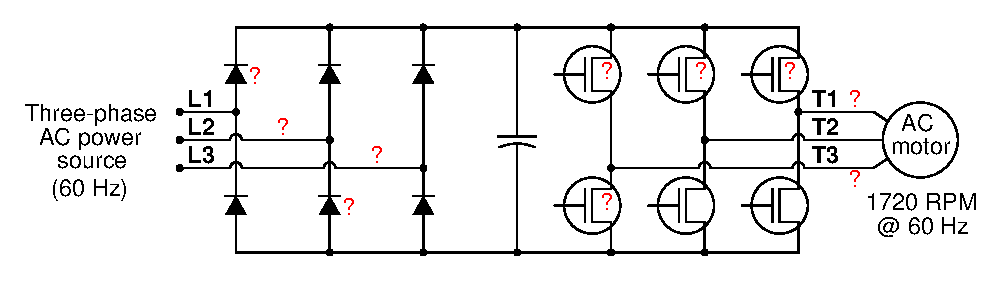
\includegraphics[width=15.5cm]{i01715x01.eps}$$

$$\includegraphics[width=15.5cm]{i01715x02.eps}$$

Use conventional flow notation to show current direction (a ``positive'' current flowing from power source to motor, and a ``negative'' current flowing from motor to power source).  If there is no current going through a labeled wire or component, just write {\bf NO} instead of drawing an arrow on the diagram.

\vskip 10pt

Also, estimate the speed of the electric motor based on the waveforms shown in the oscillographs.

\underbar{file i01715}
%(END_QUESTION)





%(BEGIN_ANSWER)

$$\includegraphics[width=15.5cm]{i01715x03.eps}$$

Speed $\approx$ 860 RPM

%(END_ANSWER)





%(BEGIN_NOTES)

%INDEX% Final Control Elements, motor: variable frequency drive

%(END_NOTES)


